\documentclass[12pt]{article}
\usepackage{amsmath}
\usepackage{graphicx}
\usepackage{hyperref}
\usepackage{listings}
\usepackage{color}
\usepackage{pythonhighlight}
\usepackage[style=apa]{biblatex} % Package APA style untuk sitasi dan dapus
\addbibresource{asset/references.bib} % Resource untuk sitasi dan dapus (file .bib)

\title{Operating System Course Report - First Half of the Semester}
\author{A class}
\date{\today}

\begin{document}

\maketitle
\newpage

\tableofcontents
\newpage

\section{Introduction}
This report summarizes the topics covered during the first half of the Operating System course. It includes theoretical concepts, practical implementations, and assignments. The course focuses on the fundamentals of operating systems, including system architecture, process management, CPU scheduling, and deadlock handling.

\section{Course Overview}
\subsection{Objectives}
The main objectives of this course are:
\begin{itemize}
    \item To understand the basic components and architecture of a computer system.
    \item To learn process management, scheduling, and inter-process communication.
    \item To explore file systems, input/output management, and virtualization.
    \item To study the prevention and handling of deadlocks in operating systems.
\end{itemize}

\subsection{Course Structure}
The course is divided into two halves. This report focuses on the first half, which covers:
\begin{itemize}
    \item Basic Concepts and Components of Computer Systems
    \item System Performance and Metrics
    \item System Architecture of Computer Systems
    \item Process Description and Control
    \item Scheduling Algorithms
    \item Process Creation and Termination
    \item Introduction to Threads
    \item File Systems
    \item Input and Output Management
    \item Deadlock Introduction and Prevention
    \item User Interface Management
    \item Virtualization in Operating Systems
\end{itemize}

\section{Topics Covered}

\subsection{Basic Concepts and Components of Computer Systems}
This section explains the fundamental components that make up a computer system, including the CPU, memory, storage, and input/output devices.

\subsubsection{Interaksi Antara \textit{Brainware}, \textit{Hardware}, dan \textit{Software}}

\subsubsection*{\textit{Brainware}}
\hspace{0.5cm} \textit{Brainware} adalah orang yang menggunakan, menjalankan, memanfaatkan, dan mengoperasikan perangkat komputer. Istilah \textit{brainware} lebih sering ditujukan kepada pengguna komputer yang mampu mengoperasikan komputer dengan canggih, baik dari segi perangkat lunak (\textit{software}) maupun perangkat keras (\textit{hardware}) (\cite{brainwareKompas}).

\subsubsection*{Jenis-Jenis \textit{Brainware}}
\hspace{0.5cm} Dalam bidang teknologi dan komputer, terdapat beragam jenis pekerjaan, masing-masing dengan peran dan tanggung jawab yang berbeda. Di bawah ini, terdapat penjelasan secara singkat:
\begin{itemize}
    \item \textbf{\textit{Project Manager}}
    \\Jenis \textit{brainware} ini bertanggung jawab untuk merencanakan, mengoordinasikan, dan mengawasi proyek teknologi dari awal hingga akhir.
    \item \textbf{Teknisi Komputer}
    \\Individu yang ahli dalam memperbaiki, memelihara, dan memasang perangkat keras dan jaringan.
    \item \textbf{Operator}
    \\Operator adalah pengguna yang mengoperasikan sistem komputer atau perangkat lunak untuk melakukan tugas-tugas tertentu.
    \item \textbf{\textit{Database Administrator}}
    \\\textit{Database Administrator} biasanya melakukan pencadangan dan pemulihan data, mengelola izin akses, dan memastikan basis data beroperasi secara optimal.
\end{itemize}

Demikianlah penjelasan tentang jenis-jenis \textit{brainware} (\cite{brainwarecmlabs}).

\subsubsection*{Hubungan antara \textit{Brainware}, \textit{Hardware}, dan \textit{Software}}
\hspace{0.5cm} Agar dapat berfungsi secara normal, komputer harus memiliki perangkat keras dan perangkat lunak. Perangkat lunak memberikan nilai fungsional pada perangkat keras.

Namun, adanya \textit{brainware} juga sangat penting. \textit{Brainware} memberikan nilai tambahan pada komputer sehingga memiliki nilai operasional. Tanpa \textit{brainware}, komputer akan menjadi robot yang tidak memiliki nilai operasional (\cite{interaksi3ware}).

Jadi, interaksi komputer tidak hanya pada perangkatnya saja, tetapi juga harus diperhatikan dari nilai operasionalnya.

\subsection{System Performance and Metrics}
This section introduces various system performance metrics used to measure the efficiency of a computer system, including throughput, response time, and utilization.

\subsection{System Architecture of Computer Systems}
Describes the architecture of modern computer systems, focusing on the interaction between hardware and the operating system.

\subsection{Process Description and Control}
Processes are a central concept in operating systems. This section covers:
\begin{itemize}
    \item Process states and state transitions
    \item Process control block (PCB)
    \item Context switching
\end{itemize}

\subsection{Scheduling Algorithms}
This section covers:
\begin{itemize}
    \item First-Come, First-Served (FCFS)
    \item Shortest Job Next (SJN)
    \item Round Robin (RR)
\end{itemize}
It explains how these algorithms are used to allocate CPU time to processes.

\subsection{Process Creation and Termination}
Details how processes are created and terminated by the operating system, including:
\begin{itemize}
    \item Process spawning
    \item Process termination conditions
\end{itemize}

\subsection{Introduction to Threads}
This section introduces the concept of threads and their relation to processes, covering:
\begin{itemize}
    \item Single-threaded vs. multi-threaded processes
    \item Benefits of multithreading
\end{itemize}

\begin{figure}[h]
    \centering
    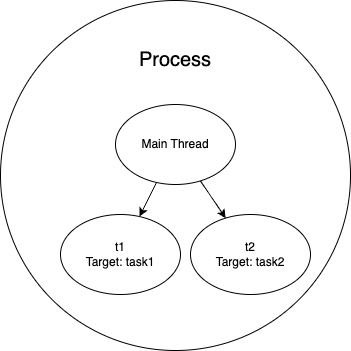
\includegraphics[width=0.5\textwidth]{asset/example.png}  % Sesuaikan nama file dan ukurannya
    \caption{Ini adalah gambar contoh dari multithreading.}
    \label{fig:contoh_gambar}
\end{figure}

Seperti yang terlihat pada Gambar \ref{fig:contoh_gambar}, inilah cara menambahkan gambar dengan keterangan.

\subsection{File Systems}
File systems provide a way for the operating system to store, retrieve, and manage data. This section explains:
\begin{itemize}
    \item File system structure
    \item File access methods
    \item Directory management
\end{itemize}

\subsection{Input and Output Management}
Input and output management is key for handling the interaction between the system and external devices. This section includes:
\begin{itemize}
    \item Device drivers
    \item I/O scheduling
\end{itemize}

\subsection{Deadlock Introduction and Prevention}
Explores the concept of deadlocks and methods for preventing them:
\begin{itemize}
    \item Deadlock conditions
    \item Deadlock prevention techniques
\end{itemize}

\subsection{User Interface Management}
This section discusses the role of the operating system in managing the user interface. Topics covered include:
\begin{itemize}
    \item Graphical User Interface (GUI)
    \item Command-Line Interface (CLI)
    \item Interaction between the user and the operating system
\end{itemize}

\subsection{Virtualization in Operating Systems}
Virtualization allows multiple operating systems to run concurrently on a single physical machine. This section explores:
\begin{itemize}
    \item Concept of virtualization
    \item Hypervisors and their types
    \item Benefits of virtualization in modern computing
\end{itemize}

\section{Assignments and Practical Work}
\subsection{Assignment 1: Process Scheduling}
Students were tasked with implementing various process scheduling algorithms (e.g., FCFS, SJN, and RR) and comparing their performance under different conditions.
\subsubsection{Group 1}
\subsubsection*{Soal}

Diberikan 4 proses dengan \textit{burst time} dan \textit{arrival time} sebagai berikut:

\begin{center}
    \begin{tabular}{|c|c|c|}
        \hline
        \textit{\textbf{Process}} & \textit{\textbf{Burst Time}} & \textit{\textbf{Arrival Time}} \\
        \hline
        P1 & 9 & 0 \\
        P2 & 3 & 1 \\
        P3 & 7 & 2 \\
        P4 & 2 & 3 \\
        \hline
    \end{tabular}
\end{center}

Hitunglah \textit{waiting time} (WT) dan \textit{average waiting time} (AWT) untuk algoritma berikut:

\begin{itemize}
    \item \textit{First-Come, First-Served} (FCFS)
    \item \textit{Round Robin} (RR) dengan \textit{Time Quantum} = 2
    \item \textit{Shortest Job First} (SJF)
\end{itemize}

Urutkan algoritma berdasarkan rata-rata waktu tunggu yang paling cepat.

\subsubsection*{Jawaban}

\textbf{FCFS}:
\begin{python}
process = ['P1', 'P2', 'P3', 'P4']
burst_time = [9, 3, 7, 2]
arrival_time = [0, 1, 2, 3]

def fcfs(process, burst_time, arrival_time):
    n = len(process)
    wt = [0] * n
    service_time = [0] * n
    
    for i in range(1, n):
        service_time[i] = service_time[i - 1] + burst_time[i - 1]
        wt[i] = service_time[i] - arrival_time[i]
        if wt[i] < 0:
            wt[i] = 0
    
    awt = sum(wt) / n
    return wt, awt

wt_fcfs, awt_fcfs = fcfs(process, burst_time, arrival_time)
print("FCFS Waiting Time: ", wt_fcfs)
print("FCFS Average Waiting Time: ", awt_fcfs)
\end{python}
\textit{Output}:
\begin{itemize}
    \item FCFS WT: [0, 8, 10, 16] (WT dari P1–P4 berturut-turut)
    \item FCFS AWT: 8.5
\end{itemize}

\textbf{RR, \textit{Time Quantum} = 2}:
\begin{python}
def round_robin(process, burst_time, arrival_time, time_quantum):
    n = len(process)
    rem_bt = burst_time[:]
    wt = [0] * n
    t = 0  # Current time
    
    while True:
        done = True
        for i in range(n):
            if rem_bt[i] > 0:
                done = False
                if rem_bt[i] > time_quantum:
                    t += time_quantum
                    rem_bt[i] -= time_quantum
                else:
                    t += rem_bt[i]
                    wt[i] = t - burst_time[i] - arrival_time[i]
                    rem_bt[i] = 0
        if done:
            break
    
    awt = sum(wt) / n
    return wt, awt

time_quantum = 2
wt_rr, awt_rr = round_robin(process, burst_time, arrival_time, time_quantum)
print("RR Waiting Time:", wt_rr)
print("RR Average Waiting Time:", awt_rr)
\end{python}
\textit{Output}:
\begin{itemize}
    \item RR (Q = 2) WT: [12, 7, 11, 3] (WT dari P1–P4 berturut-turut)
    \item RR (Q = 2) AWT: 8.25
\end{itemize}

\textbf{SJF}:
\begin{python}
def sjf(process, burst_time, arrival_time):
    n = len(process)
    wt = [0] * n
    bt = burst_time[:]
    at = arrival_time[:]
    
    completed = 0
    t = 0
    min_bt = 0
    shortest = 0
    check = False
    
    while completed != n:
        for i in range(n):
            if at[i] <= t and bt[i] > 0 and (not check or bt[i] < bt[shortest]):
                shortest = i
                min_bt = bt[i]
                check = True
                
        if not check:
            t += 1
            continue
        
        bt[shortest] -= 1
        min_bt -= 1
        if bt[shortest] == 0:
            completed += 1
            check = False
            finish_time = t + 1
            wt[shortest] = finish_time - burst_time[shortest] - at[shortest]
            if wt[shortest] < 0:
                wt[shortest] = 0
        t += 1
    
    awt = sum(wt) / n
    return wt, awt

wt_sjf, awt_sjf = sjf(process, burst_time, arrival_time)
print("SJF Waiting Time:", wt_sjf)
print("SJF Average Waiting Time:", awt_sjf)
\end{python}
\textit{Output}:
\begin{itemize}
    \item SJF WT: [12, 0, 4, 1] (WT dari P1–P4 berturut-turut)
    \item SJF AWT: 4.25
\end{itemize}

Dengan demikian, urutan algoritma berdasarkan rata-rata waktu tunggu (AWT) yang paling cepat adalah:
\begin{itemize}
    \item SJF
    \item RR (Q = 2)
    \item FCFS
\end{itemize}

\subsection{Assignment 2: Deadlock Handling}
In this assignment, students were asked to simulate different deadlock scenarios and explore various prevention methods.

\subsection{Assignment 3: Multithreading and Amdahl's Law}
This assignment involved designing a multithreading scenario to solve a computationally intensive problem. Students then applied **Amdahl's Law** to calculate the theoretical speedup of the program as the number of threads increased.
\subsubsection{Group 1}
\subsubsection*{Soal}

Pada sistem komputasi modern, penggunaan \textit{multithreading} sering kali dite-rapkan untuk mempercepat eksekusi program dengan cara menjalankan beberapa bagian program secara paralel. Efektivitas dari pendekatan ini dapat diukur menggunakan Hukum Amdahl. 

Diketahui persamaan Hukum Amdahl sebagai berikut:

\[
S_{max} = \frac{1}{(1 - P) + \frac{P}{N}}
\]

keterangan:
\begin{itemize}
    \item \(S_{max}\) adalah percepatan maksimum yang dapat dicapai,
    \item \(P\) adalah persentase bagian dari program yang dapat diparalelkan,
    \item \(N\) adalah jumlah \textit{threads} atau prosesor yang digunakan.
\end{itemize}

Berikut ini adalah tiga skenario yang harus diselesaikan:

1. Sebuah program memiliki 70\% bagian yang dapat diparalelkan (\(P = 0.7\)). Tentukan percepatan maksimum (\(S_{max}\)) jika program dijalankan dengan:
\begin{itemize}
    \item 2 \textit{threads},
    \item 4 \textit{threads},
    \item 8 \textit{threads}.
\end{itemize}

2. Jika suatu program dapat diparalelkan sebesar 85\% (\(P = 0.85\)), berapa jumlah minimum \textit{threads} yang diperlukan untuk mencapai percepatan lima kali lipat dari waktu eksekusi serial (\(S_{max} = 5\))?

3. Jelaskan secara singkat, apakah selalu lebih baik menggunakan lebih banyak \textit{threads}? Berdasarkan Hukum Amdahl, berikan alasan mengapa penggunaan \textit{multithreading} kadang tidak memberikan percepatan yang signifikan.

\subsubsection*{Jawaban}

\textbf{1. Menghitung percepatan maksimum (\(S_{max}\))}:

\begin{python}
P = 0.7

def amdahls_law(P, N):
    return 1 / ((1 - P) + (P / N))

threads = [2, 4, 8]
for N in threads:
    S_max = amdahls_law(P, N)
    print(f"Percepatan maksimum untuk {N} threads: {S_max:.2f}")
\end{python}
\textit{Output}:
\begin{itemize}
    \item Untuk 2 \textit{threads}, \(S_{max} \approx 1.75\)
    \item Untuk 4 \textit{threads}, \(S_{max} \approx 2.61\)
    \item Untuk 8 \textit{threads}, \(S_{max} \approx 3.43\)
\end{itemize}

\textbf{2. Mencari jumlah minimum \textit{threads} untuk mencapai percepatan lima kali lipat}:

\begin{python}
from math import ceil

P = 0.85
S_target = 5

def find_min_threads(P, S_target):
    N = 1
    while True:
        S_max = amdahls_law(P, N)
        if S_max >= S_target:
            return N
        N += 1

min_threads = find_min_threads(P, S_target)
print(f"Jumlah minimum threads untuk mencapai percepatan lima kali lipat: {min_threads}")
\end{python}
\textit{Output}: Jumlah minimum \textit{threads} yang diperlukan adalah 10.

\textbf{3. Mengapa penggunaan lebih banyak \textit{threads} tidak selalu efektif?}

\textit{Multithreading} memiliki batas percepatan yang dapat dicapai. Berdasarkan Hukum Amdahl, jika persentase bagian program yang tidak dapat diparalelkan (\(1 - P\)) cukup besar, maka menambahkan lebih banyak \textit{threads} tidak akan memberikan percepatan yang signifikan. Bahkan dengan jumlah \textit{threads} yang sangat besar, bagian program yang tidak bisa diparalelkan akan tetap menjadi penghalang utama untuk mencapai percepatan yang tinggi.

\subsection{Assignment 4: Simple Command-Line Interface (CLI) for User Interface Management}
Students were tasked with creating a simple **CLI** for user interface management. The CLI should support basic commands such as file manipulation (creating, listing, and deleting files), process management, and system status reporting.
\subsubsection{Group 1}
\subsubsection*{Soal}
Mahasiswa diminta untuk membuat \textit{Simple Command-Line Interface} (CLI) untuk manajemen antarmuka pengguna. CLI ini harus mendukung perintah-perintah dasar seperti:

\begin{itemize}
    \item Manipulasi berkas (membuat, menampilkan daftar, dan menghapus berkas),
    \item Manajemen proses,
    \item Pelaporan status sistem.
\end{itemize}

Berikut ini adalah spesifikasi tugasnya:

1. \textbf{Manipulasi berkas:}
    \begin{itemize}
        \item \texttt{buat\_berkas <nama\_berkas>} - Membuat berkas baru dengan nama yang diberikan.
        \item \texttt{daftar\_berkas} - Menampilkan daftar semua berkas di direktori saat ini.
        \item \texttt{hapus\_berkas <nama\_berkas>} - Menghapus berkas dengan nama yang diberikan.
    \end{itemize}

2.  \textbf{Manajemen proses:}
    \begin{itemize}
        \item \texttt{daftar\_proses} - Menampilkan daftar semua proses yang sedang berjalan.
        \item \texttt{hentikan\_proses <PID>} - Menghentikan proses berdasarkan \textit{Process ID} (PID).
    \end{itemize}

3.  \textbf{Pelaporan status sistem:}
    \begin{itemize}
        \item \texttt{status\_sistem} - Menampilkan informasi tentang penggunaan CPU, memori, dan ruang disk.
    \end{itemize}

Mahasiswa harus mengimplementasikan fungsi-fungsi ini dalam bahasa pemrograman Python dan memastikan semua perintah dapat dijalankan dari \textit{command-line}.

\textbf{Tugas:}
\begin{itemize}
    \item Implementasikan semua fungsi di atas menggunakan Python.
    \item Jelaskan bagaimana setiap perintah dieksekusi dan berikan contoh keluaran dari setiap perintah.
\end{itemize}

\subsubsection*{Jawaban}

\textbf{Contoh implementasi Python untuk perintah-perintah dasar CLI:}

\begin{python}
import os # Operating System
import psutil # Process and System Utilities

# Fungsi untuk membuat berkas baru
def buat_berkas(nama_berkas):
    with open(nama_berkas, 'w') as f:
        f.write('Berkas berhasil dibuat.\n')
    print(f'Berkas "{nama_berkas}" telah dibuat.')

# Fungsi untuk menampilkan daftar berkas di direktori saat ini
def daftar_berkas():
    files = os.listdir('.')
    for file in files:
        print(file)

# Fungsi untuk menghapus berkas
def hapus_berkas(nama_berkas):
    if os.path.exists(nama_berkas):
        os.remove(nama_berkas)
        print(f'Berkas "{nama_berkas}" telah dihapus.')
    else:
        print(f'Berkas "{nama_berkas}" tidak ditemukan.')

# Fungsi untuk menampilkan daftar proses yang berjalan
def daftar_proses():
    for proc in psutil.process_iter(['pid', 'name']):
        print(f"PID: {proc.info['pid']}, Nama Proses: {proc.info['name']}")

# Fungsi untuk menghentikan proses berdasarkan PID
def hentikan_proses(pid):
    try:
        p = psutil.Process(pid)
        p.terminate()
        print(f'Proses dengan PID {pid} telah dihentikan.')
    except psutil.NoSuchProcess:
        print(f'Tidak ada proses dengan PID {pid}.')

# Fungsi untuk menampilkan status sistem
def status_sistem():
    print(f'Penggunaan CPU: {psutil.cpu_percent()}%')
    print(f'Penggunaan Memori: {psutil.virtual_memory().percent}%')
    print(f'Penggunaan Disk: {psutil.disk_usage("/").percent}%')
\end{python}
\textbf{Contoh Penggunaan:}

\begin{itemize}
    \item \texttt{buat\_berkas("contoh.txt")} akan membuat berkas bernama \texttt{contoh.txt}.
    \item \texttt{daftar\_berkas()} akan menampilkan semua berkas di direktori saat ini.
    \item \texttt{hapus\_berkas("contoh.txt")} akan menghapus berkas bernama
    \\\texttt{contoh.txt}.
    \item \texttt{daftar\_proses()} akan menampilkan semua proses yang sedang berjalan.
    \item \texttt{hentikan\_proses(12345)} akan menghentikan proses dengan PID 12345.
    \item \texttt{status\_sistem()} akan menampilkan penggunaan CPU, memori, dan ruang disk.
\end{itemize}

\subsection{Assignment 5: File System Access}
In this assignment, students implemented file system access routines, including:
\begin{itemize}
    \item File creation and deletion
    \item Reading from and writing to files
    \item Navigating directories and managing file permissions
\end{itemize}

\subsubsection{Group 1}
\subsubsection*{Soal}

Dalam tugas ini, mahasiswa diminta untuk mengimplementasikan beberapa fungsi akses sistem berkas, yang meliputi:

\begin{itemize}
    \item Pembuatan dan penghapusan berkas,
    \item Membaca dari dan menulis ke dalam berkas,
    \item Menavigasi direktori dan mengelola izin berkas.
\end{itemize}

\textbf{Spesifikasi tugas:}

1. \textbf{Pembuatan dan penghapusan berkas:}
    \begin{itemize}
        \item Implementasikan fungsi untuk membuat berkas baru di direktori yang ditentukan oleh pengguna.
        \item Implementasikan fungsi untuk menghapus berkas yang ada.
    \end{itemize}

2. \textbf{Membaca dan menulis berkas:}
    \begin{itemize}
        \item Buat fungsi untuk membaca isi berkas.
        \item Buat fungsi untuk menulis data baru ke dalam berkas yang ada.
    \end{itemize}

3. \textbf{Navigasi direktori dan izin berkas:}
    \begin{itemize}
        \item Buat fungsi untuk berpindah antara direktori di sistem file.
        \item Buat fungsi untuk menampilkan dan mengubah izin berkas (\textit{file permissions}).
    \end{itemize}

\textbf{Tugas:}
\begin{itemize}
    \item Implementasikan fungsi-fungsi di atas menggunakan Python.
    \item Sertakan contoh penggunaan dari setiap fungsi yang telah dibuat.
\end{itemize}

\subsubsection*{Jawaban}

\textbf{Contoh implementasi Python untuk fungsi-fungsi akses sistem berkas:}

\begin{python}
import os

# Fungsi untuk membuat berkas baru
def buat_berkas(nama_berkas):
    with open(nama_berkas, 'w') as f:
        f.write('Ini adalah berkas baru.\n')
    print(f'Berkas "{nama_berkas}" telah dibuat.')

# Fungsi untuk menghapus berkas
def hapus_berkas(nama_berkas):
    if os.path.exists(nama_berkas):
        os.remove(nama_berkas)
        print(f'Berkas "{nama_berkas}" telah dihapus.')
    else:
        print(f'Berkas "{nama_berkas}" tidak ditemukan.')

# Fungsi untuk membaca isi berkas
def baca_berkas(nama_berkas):
    if os.path.exists(nama_berkas):
        with open(nama_berkas, 'r') as f:
            isi = f.read()
            print(isi)
    else:
        print(f'Berkas "{nama_berkas}" tidak ditemukan.')

# Fungsi untuk menulis ke berkas
def tulis_berkas(nama_berkas, data):
    with open(nama_berkas, 'a') as f:
        f.write(data + '\n')
    print(f'Data telah ditulis ke berkas "{nama_berkas}".')

# Fungsi untuk menavigasi direktori
def pindah_direktori(direktori):
    try:
        os.chdir(direktori)
        print(f'Berpindah ke direktori: {os.getcwd()}')
    except FileNotFoundError:
        print(f'Direktori "{direktori}" tidak ditemukan.')

# Fungsi untuk mengubah izin berkas
def ubah_izin(nama_berkas, izin):
    if os.path.exists(nama_berkas):
        os.chmod(nama_berkas, izin)
        print(f'Izin berkas "{nama_berkas}" telah diubah.')
    else:
        print(f'Berkas "{nama_berkas}" tidak ditemukan.')
\end{python}
\textbf{Contoh Penggunaan:}

\begin{itemize}
    \item \texttt{buat\_berkas("file\_contoh.txt")} akan membuat berkas bernama
    \\\texttt{file\_contoh.txt}.
    \item \texttt{hapus\_berkas("file\_contoh.txt")} akan menghapus berkas bernama \texttt{file\_contoh.txt}.
    \item \texttt{baca\_berkas("file\_contoh.txt")} akan menampilkan isi dari
    \\\texttt{file\_contoh.txt}.
    \item \texttt{tulis\_berkas("file\_contoh.txt", "Data baru")} akan menulis \texttt{Data baru} ke dalam \texttt{file\_contoh.txt}.
    \item \texttt{pindah\_direktori("/home/user/direktori")} akan berpindah ke direktori \texttt{/home/user/direktori}.
    \item \texttt{ubah\_izin("file\_contoh.txt", 0o755)} akan mengubah izin berkas \texttt{file\_contoh.txt} menjadi 755.
\end{itemize}
Arti 0o755:
\begin{itemize}
    \item 0o menunjukkan bahwa angka berikutnya adalah dalam sistem oktal.
    \item 7 (untuk pemilik): 4 (baca) + 2 (tulis) + 1 (eksekusi) = 7. Jadi, pemilik dapat membaca, menulis, dan mengeksekusi berkas.
    \item 5 (untuk grup): 4 (baca) + 1 (eksekusi) = 5. Jadi, anggota grup dapat membaca dan mengeksekusi berkas, tetapi tidak dapat menulis.
    \item 5 (untuk lainnya): 4 (baca) + 1 (eksekusi) = 5. Jadi, pengguna lain dapat membaca dan mengeksekusi berkas, tetapi tidak dapat menulis.
\end{itemize}

\section{Conclusion}
The first half of the course introduced core operating system concepts, including process management, scheduling, multithreading, and file system access. These topics provided a foundation for more advanced topics to be covered in the second half of the course.

\newpage % Membuat halaman baru untuk dapus/references
\addcontentsline{toc}{section}{References} % Menambahkan section References ke toc (Table of Contents) tanpa dimasukkan ke daftar section yang telah ada (tanpa diawali dengan angka)
\printbibliography{} % Menampilkan dapus APA style

\end{document}